\section{Betaling}

I dette afsnit vil arkitekturen for widgettypen Betaling blive præsenteret. Dette vil ligge grundlag for at en uddybende beskrivelse af hvordan widget'en er designet og implementeret. 

\begin{figure}[H]
    \centering
    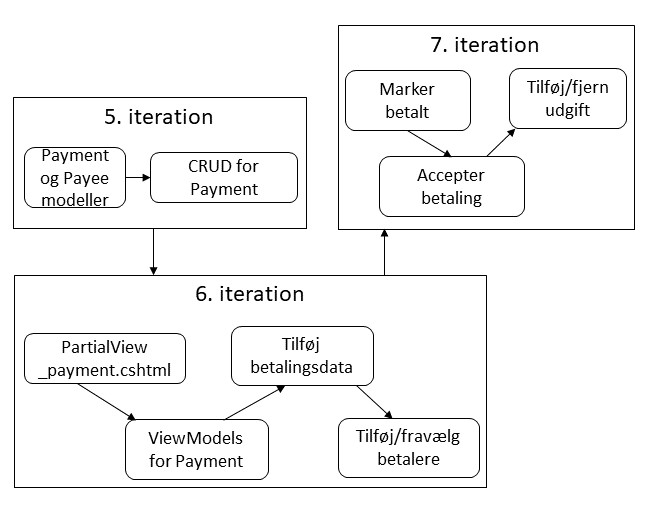
\includegraphics[width=\linewidth]{09_Arkitektur/Payment/Images/iteraionerCropped1.jpg}
    \caption{Der er blevet arbejdet på Betaling i de sidste uger i forløbet. Denne funktionalitet har kunnet blive implementeret direkte som en widget, og består også af en del JavaScript.}
    \label{fig:paymentIterations}
\end{figure}

\jonathan{Find ud af om det kan gøres lidt mindre når vi er ved at være færdige, så det kan være på en side}

Denne widget er vigtig for WePlanner på den måde at det i gruppe sammenhænge ofte er essentielt at kunne notere forskellige beløb der er blevet lagt ud for, og at kunne få et overblik over hvad andre har lagt ud for, så man kan få dem betalt.

\subsection{Data view}

En betaling består i WePlanners database af 2 modeller: Payment og Payees. For en Payment er der flere Payees, hvor Payees er Users, med ekstra attributter. De Users der skal være mulige at være Payees, skal være a typen GroupUsers, hvilket er en Model der er lavet i sammengængen med opsættelse af Groups. På baggrund af dette er dataen for Betalinger sat op på følgende måde.

\begin{figure}[H]
    \centering
    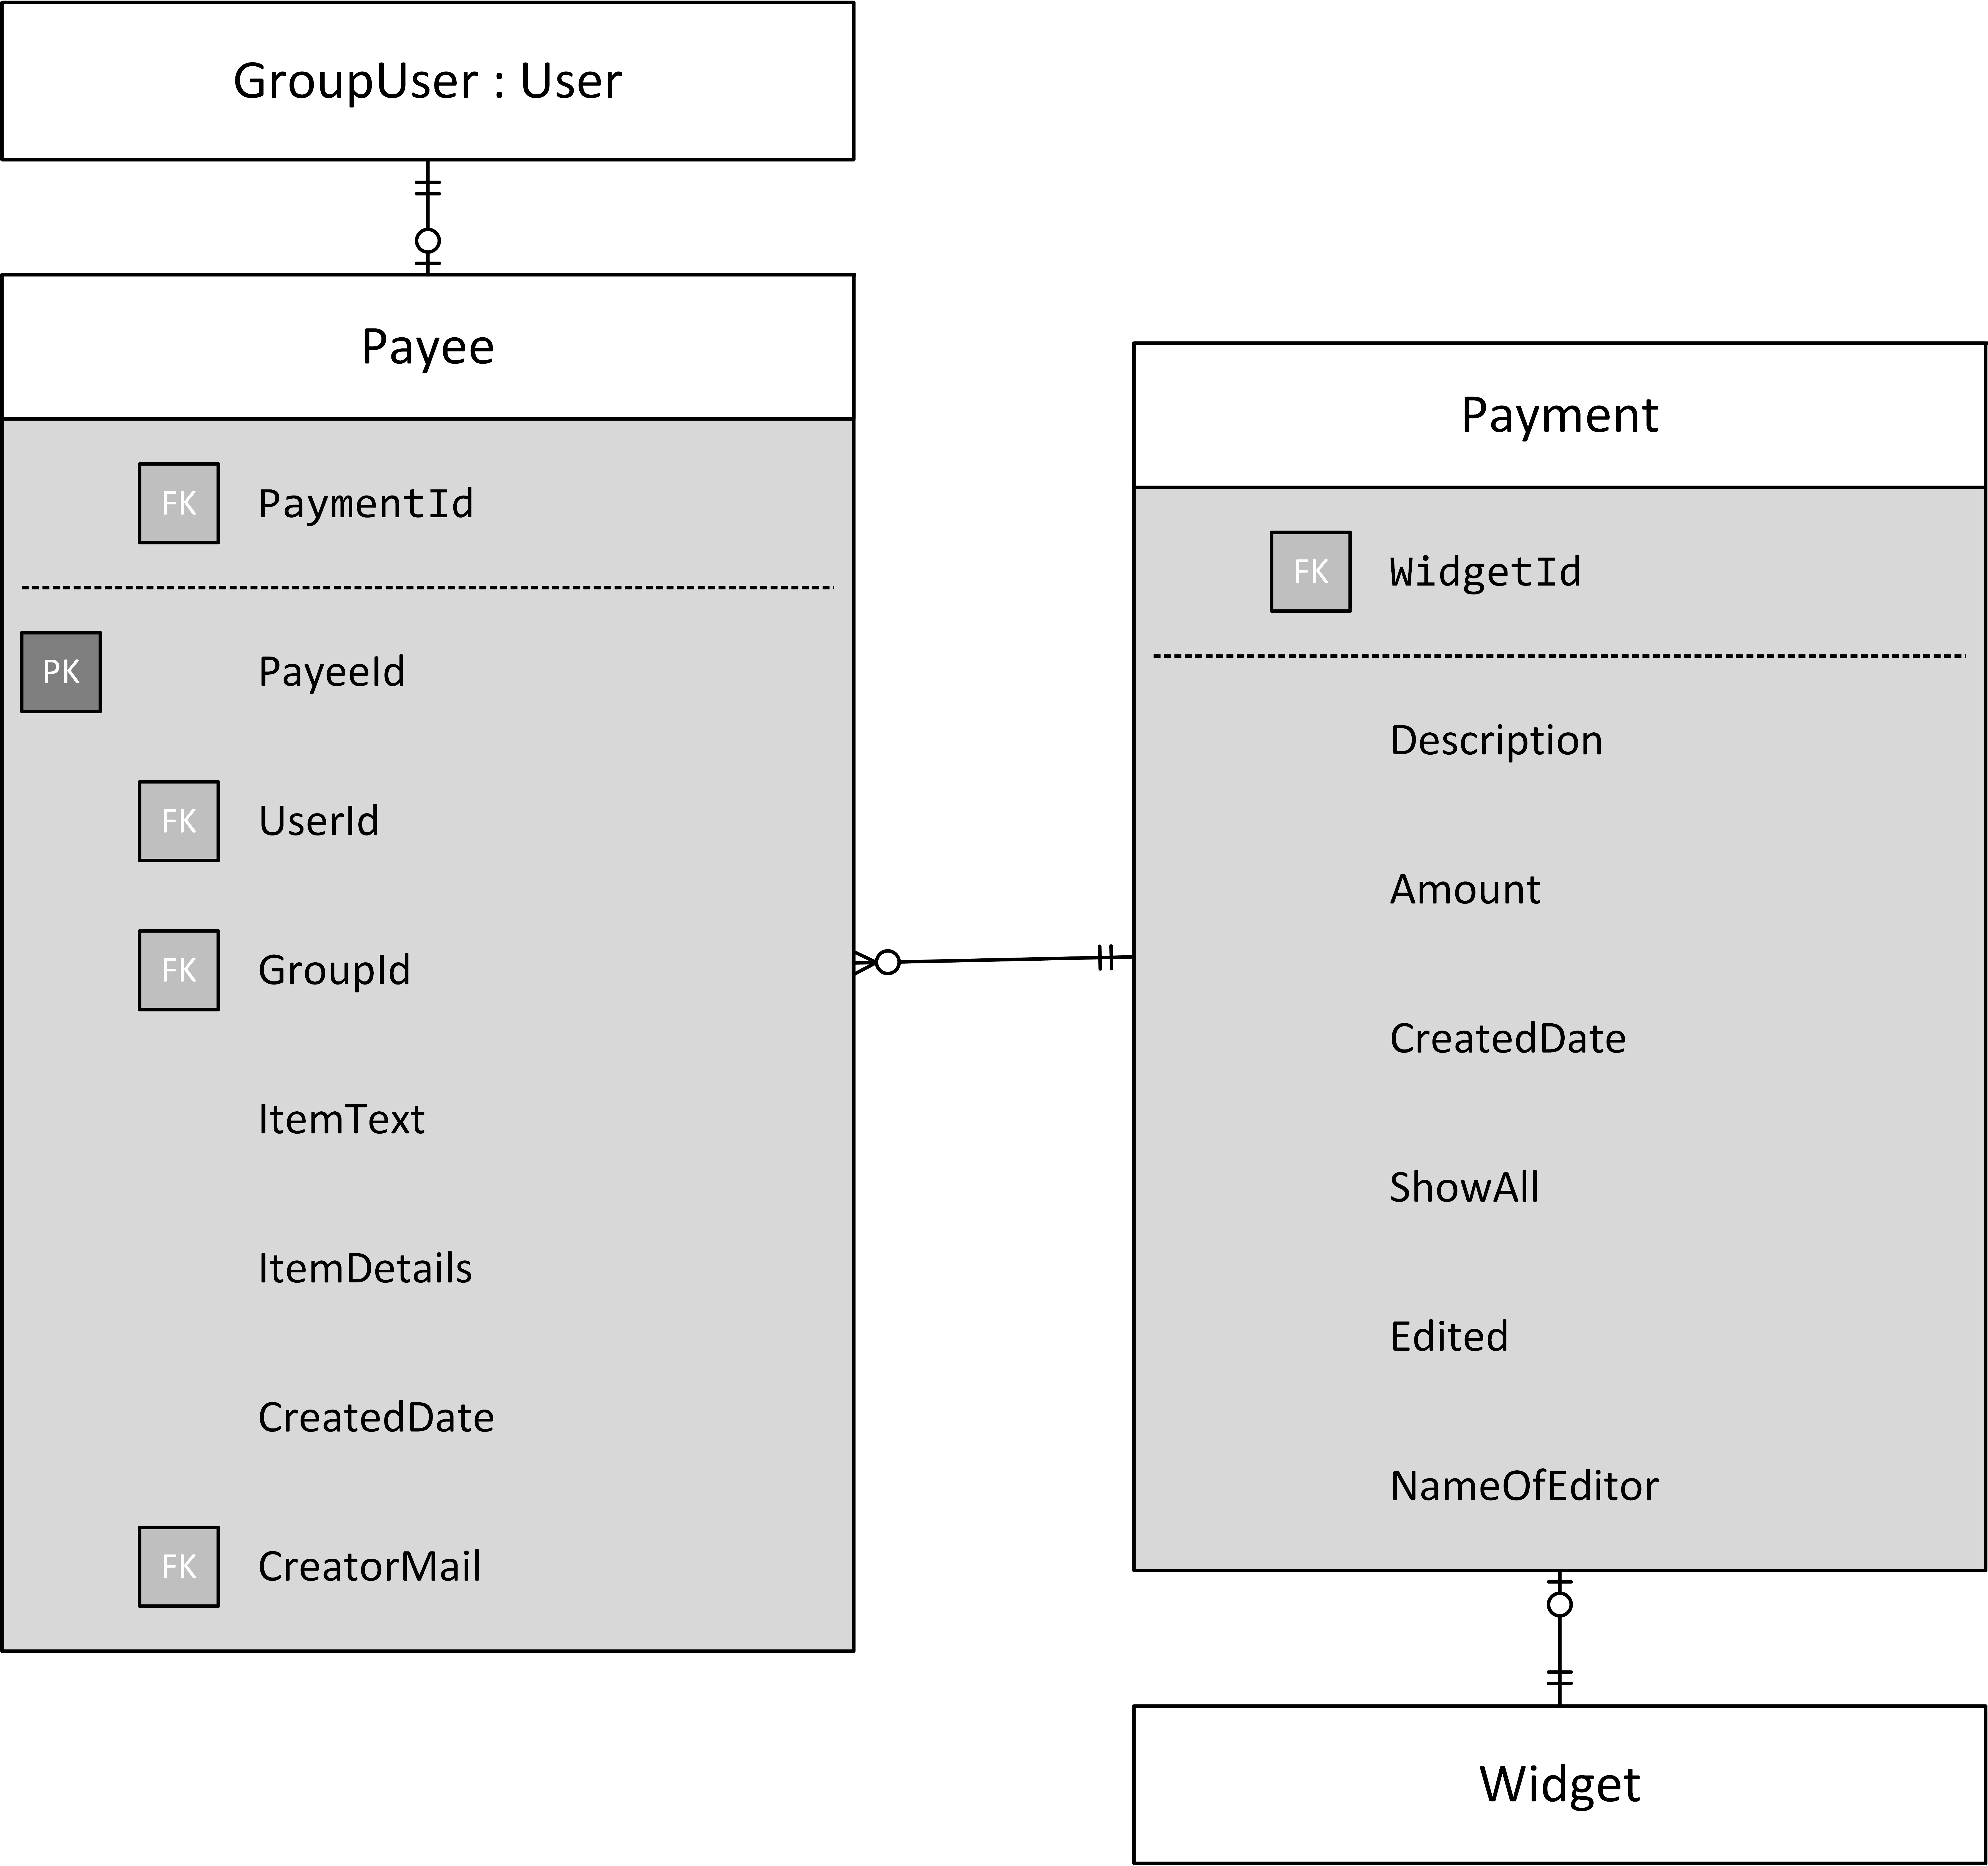
\includegraphics[width=\linewidth]{09_Arkitektur/Payment/Images/partialERDBetaling.png}
    \caption{Diagrammet viser dele af entitetsrelationerne mellem Payment og Payees, hvor det ses at Payment har en Widget, hvilket er vigtigt for WePlanners dashboard, som er gjort generelt for alle typer af Widgets.}
    \label{fig:betalingERD}
\end{figure}

For ovenstående Entity Relation diagram gælder det at en Payee har en GroupUser, hvor payee får alle denss vigtige brugerinformationer fra. Gennem GroupUser kan dder tilgås User, som der kan fås UserId, Email, Name etc. Disse bliver anvendt en del i Betaling, da det giver mere konfidentialitet at have information om brugeren, når der deles information om penge. Det fulde ER diagram kan ses i bilag om arkitektur for Betaling\cite{paymentPartERD}.

\subsection{Logical view}

Betalingen i WePlanner har lidt den samme funktionalitet som MobilePays underdel WeShare\cite{weShare}, som gør det muligt at dele udgifter med hindanden. Formålet med prototypen for WePlanner er på en måde at samle mange funktionaliteter et sted, hvor af en af funktionaliteterne er en slags WeShare. I fremtidige iterationer kunne det være en idé at undersøge muligheden for at kunne gå sammen med MobilePay of WeShare.\\

\noindent På nedenstående figur \ref{fig:paymentFunctionality}, ses hvad der kan gøres ud fra en Payment.

\begin{figure}[H]
    \centering
    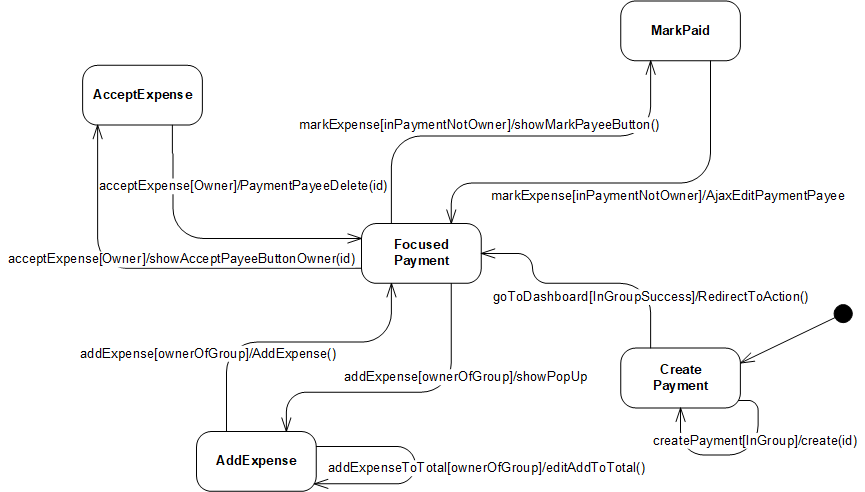
\includegraphics[width=\linewidth]{09_Arkitektur/Payment/Images/Payment_STM.png}
    \caption{Det ses at man ud fra en Payment kan Markerer som betalt, Accepter betaling og tilføj ny udgift. Hvordan dette gøres beskrives yderligere i design og implementering og mere detaljeret i projektets bilag.}
    \label{fig:paymentFunctionality}
\end{figure}

\jonathan{Ved ikke hvad jeg mere skal skrive... fml}